\documentclass[12pt,onecolumn,a4paper]{article}
%\usepackage[square,numbers]{natbib}  % for bib and references
%\usepackage[round]{natbib}  % for bib and references
\usepackage{hyperref}
\usepackage{caption}
\usepackage{float}
\usepackage{epsfig,graphicx,subfigure,amsthm,amsmath}
\usepackage{color,xcolor}     
\usepackage[left=0.75in,top=1in,right=0.75in,bottom=0.6in]{geometry} % Document margins
\usepackage{fontawesome}
\usepackage{soul} % for highlighting 
%\usepackage{cmbright}
\usepackage{titling}

\usepackage{natbib}
\bibliographystyle{abbrvnat}
\setcitestyle{authoryear} %Citation-related commands

\setlength{\droptitle}{-10em}
\renewcommand\maketitlehooka{%
\setlength\parindent{0pt}%
%\setcitestyle{numbers}
\definecolor{coolblack}{rgb}{0.0, 0.18, 0.39}
\begin{center}
 
\includegraphics[scale=0.3]{leth-log.png}
 \\
  \textbf{Master's Thesis Proposal\\}
  \small{Ver. 1, Ed. 2, \today}
   
%  \textbf{\\”Make the change that you want to see in the world.”}
  \end{center}

\begin{minipage}{.5\textwidth}
  \raggedright
  {
  Your name\\
  Master's Student
  \\ \vspace{.4em}
  }

\end{minipage}
\begin{minipage}{.5\textwidth}
  \raggedleft
 {
  Your Supervisor name\\
  Supervisor
  \\
  }

\end{minipage}
\par
\hrule
}

\begin{document}
\title{\vspace{-5ex}}
\date{\vspace{-5ex}}
\author{\vspace{-5ex}}
\maketitle
%%%%%%%% 
% an intro from the official form of undergraduate projects  
%%%%%%%% 
\begin{center}
    Enriching Abstractive Summarization Models With Graphs and Graph Neural Networks
\end{center}

\section{Introduction}

Natural Languages Processing (NLP) has various branches, namely Text-to-Text (T2T) Generation, Information Retrieval, or Machine Reasoning and Comprehension among others. One of the challenging tasks in T2T generation is Automatic Text Summarization. Text summarization has been studies more than seven decades and has received a great deal of community attention over the last two decades \citep{Kumar2022}, yet we are far behind the human performance in this task \citep{wafaa}.\\

Earlier developed systems were predominantly extractive while with the raise of Sequence-to-Sequence (seq2seq) models they leaned towards being abstractive\citep{Hou2018} (Fig \ref{figure:abs_ext_arch} demonstrates the architecture of these two approaches). One of the successful variation of seq2seq approaches is transformers\citep{vaswani2017}, initially designed for Machine Translation, which has contributed to higher performance in various language generation tasks. With the notion of key, query, and value, it generates a relatively rich intermediate representation. Although token level and shallow, this representation is good enough, based on the experimental results, for machine translation and perform near human level and even outperform humans in some specific circumstances\citep{Popel2020}.\\

Transformers and its variation, however, fall short in more cognitively complicated language generation tasks, namely Dialogue Management (appendix \ref{appendix:gpt}) or Text Summarization in which we have to manage long dependencies, reason over the importance of sentences and how to tailor important parts coherently and cohesively. A recent survey showed that enriching previous state-of-the-art (SOTA) models with graph neural networks (GNNs) can increase their performance \citep{salchner2022survey}.\\

GNN based approaches and SOTA models both incorporate probabilistic training and prediction with neural networks frameworks, yet GNN-based models add clear meta-knowledge about of textual data by utilizing the power of graphs. A recent research shows \citep{GNNBook-ch21-liu} five versatile graphs (text graphs, syntactic graphs, semantic graphs, knowledge graphs, and hybrid graphs) can significantly improve the performance of models in T2T generation tasks.

\begin{figure}[ht]
\centering
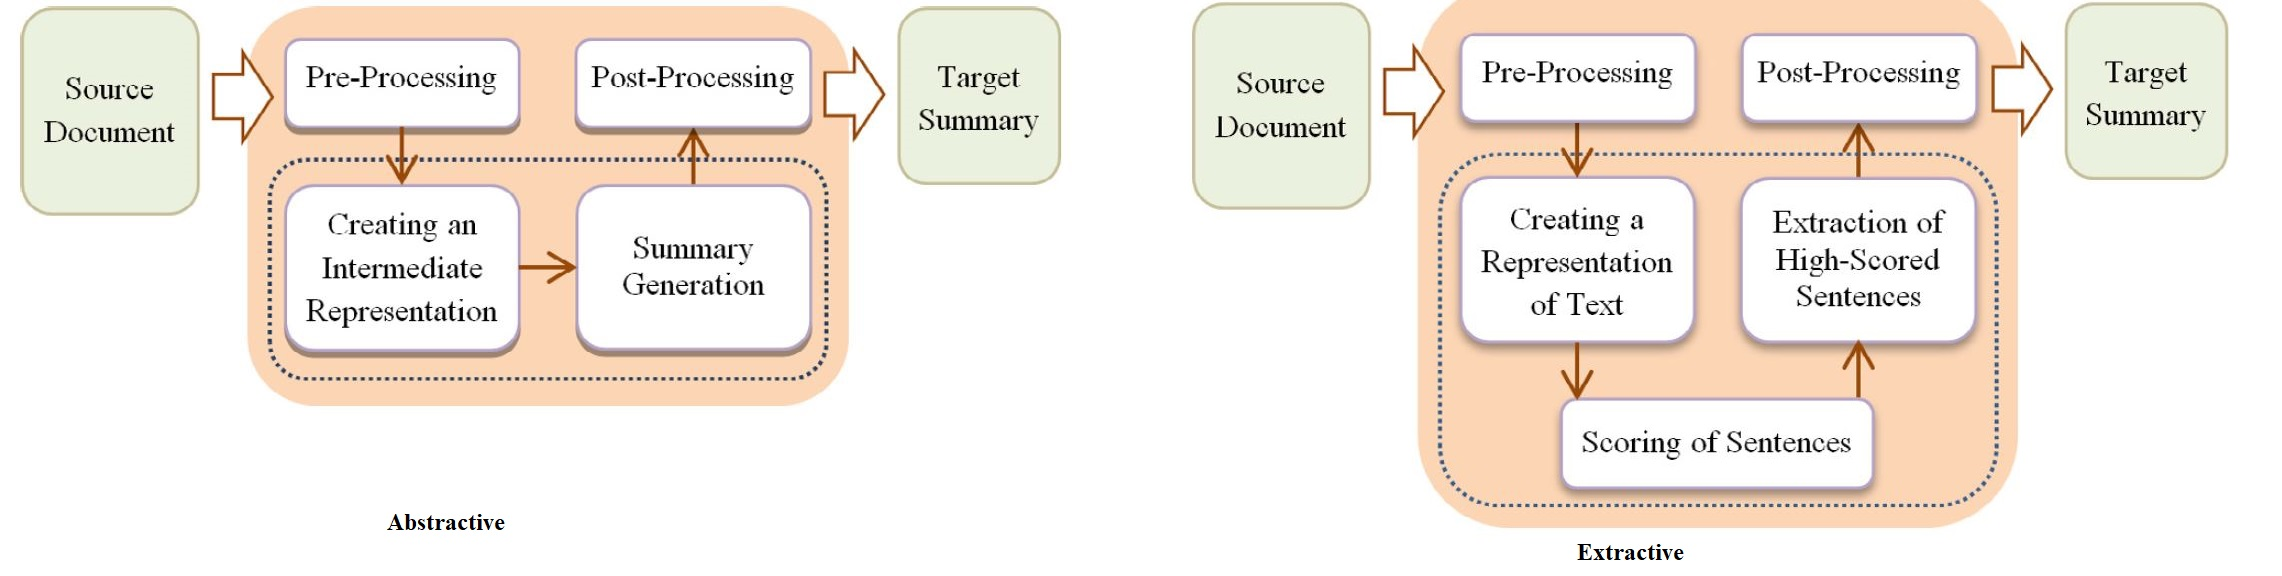
\includegraphics[width=0.8\textwidth]{Abs_Ext_architecture.jpg}
\caption{Architecture of automatic abstractive and extractive systems \cite{wafaa}}
\label{figure:abs_ext_arch}
\end{figure}

%%%%%%%%%%%%%%



\section{Literature review}
\noindent In order to incorporate GNNs in natural language processing tasks we have to answer two questions: the graph structure used for text modeling, and architecture of GNN. Five categories of graph types that we can use are alluded earlier. There are two main components in any GNN layer: aggregate and combine \citep{GNNBook-ch4-tang}. Most of the differences between various GNN architectures, namely graph convolutional networks (GCN) \citep{GCN} or Graph Attention Networks (GAT) \citep{GAT}, comes from these two important components.\\ 

Other design choices of GNN greatly depend on the task. One of them, for instance, is whether we have stand-alone or embedded design \citep{salchner2022survey}. Stand-alone models use GNNs to directly produce the summary, embedded approach, however, use GNNs as a part of a large system. HeterSumGraph \citep{wang-etal-2020-heterogeneous} as an example of stand-alone  architecture which uses three different graph nodes (word, sentence, and document nodes) to classify important sentences as the final summary.\citep{FAsum2021} recently showed that by embedding GNN in Transformers architecture, we can outperform previous models, particularly in factual consistancy metric.\\

Removed.\\




\section{Hypothesis}
\hl{The main goal in your research that you believe is the case. In another word, the idea that you have come up with that and you believe that you can prove that positive.}

\section{Objectives}
Our objectives are as follows: (1) Representing textual data with graph A and B, (2) Removed, (3) Removed (4) Removed.


\section{Research design and method}

\subsection{Data set}
\hl{Dataset section. You will briefly explain the dataset that you will be using.}.

\subsection{Approach}
\hl{
In this section, you will outline the steps necessary to achieve your hypothesis, aiming to prove it positively. It's important to note that nothing in a thesis, apart from the main goal (the Hypothesis), is considered fixed unless explicitly stated. Therefore, when explaining the approach that you believe might work, it's advisable to use hedging and qualifying statements. Avoid definitive statements like "I will certainly use FFNN to prove my hypothesis," as you may later discover that FFNN is not suitable for your setup, while another method may better serve your goal. Instead, utilize hedging language such as "In part C of my approach, I consider using FFNN, as it has been shown to be effective in many cases."}


\subsection{Implementation}
We will, in part, use PyG \footnote{https://pyg.org/p} framework which is designed to accelerate implementation of graph neural networks for NLP.

\subsection{Evaluation}

We will Measure abstraction by calculating percentage of novel n-grams in the generated summary. In order to measure how in keeping with the ground-truth is the predicted summary, We use ... \hl{Bring other metrics, if needed.}


\section{Future Directions}
Supposing this proposal come into fruition, there are several possible future works such as: \hl{Your realistic future works (not more than one paragraph).}


\section{Time Line}
\hl{Briefly and realistically sketch a schedule here.}
Summer 2023: Encoder part. ... \\
Fall 2023: Decoder part ... \\
Spring 2024: Evaluation ... \\
Summer 2024: Thesis draft, correction, defense ...
\newpage
\section{References}
\vspace*{-\baselineskip}
\setlength{\bibsep}{2pt}
\renewcommand*{\bibfont}{\scriptsize}
\renewcommand{\refname}{}
\bibliography{mybibfile.bib}
%\bibliographystyle{acl_natbib}
%\bibliographystyle{unsrtnat} % for number format
%\bibliographystyle{plainnat}

\newpage

\section{Appendix}
\appendix
\section{Inference problem in the SOTA dialouge systems}
\label{appendix:gpt}
The following prompts are experiments with ChatGPT\footnote{\href{https://openai.com/blog/chatgpt/}{ChatGPT released on November 30, 2022}} available on the Internet.
\begin{center}%
    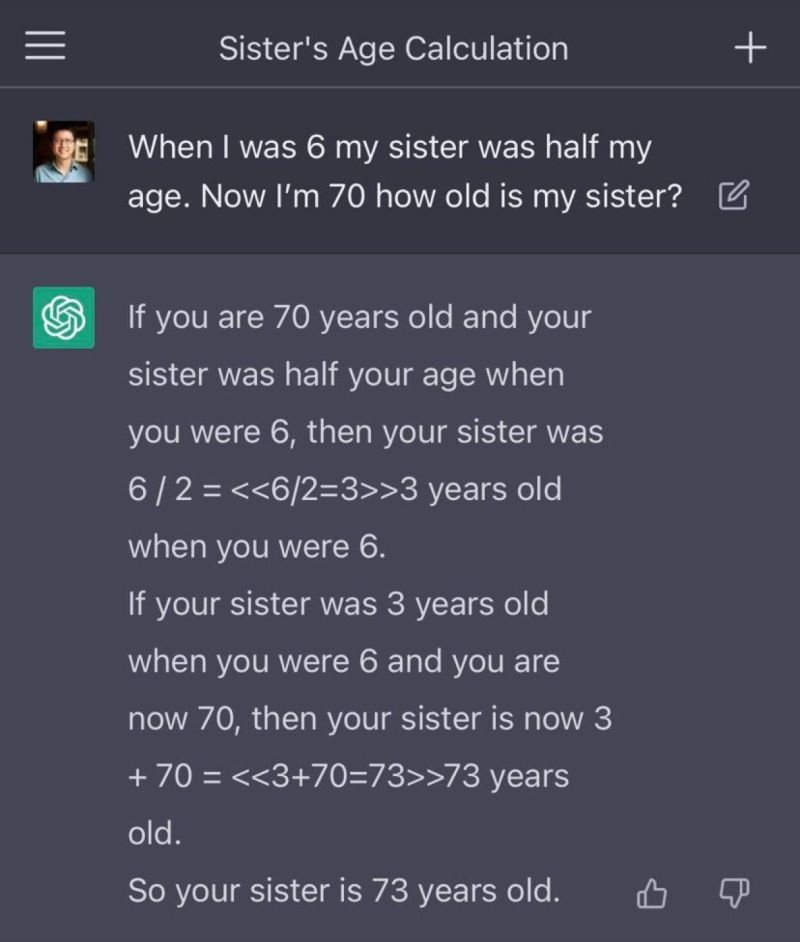
\includegraphics[width=8cm]{ChatGPT_1.png} 
    \qquad
    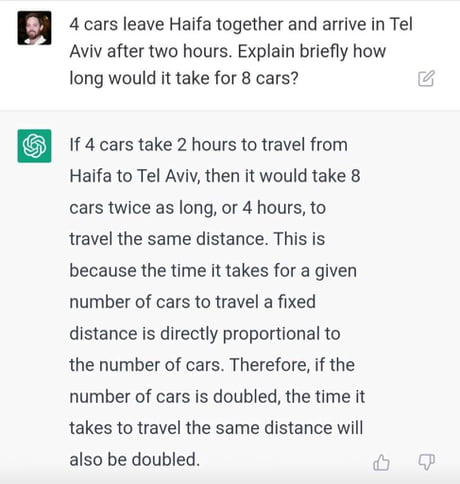
\includegraphics[width=8cm]{chatGPT_2.jpg}
\end{center}





\end{document}